\chapter{Introduction}
\begin{figure}
\centering
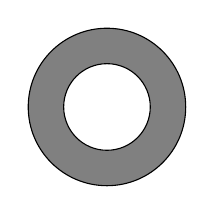
\begin{tikzpicture}[scale=.25]
  \filldraw[draw=black,fill=gray] (0,0) circle [radius=4];
      \filldraw[draw=black,fill=white] (0,0) circle [radius=2.2];
 \end{tikzpicture}      
 \hspace{.5cm}
\begin{tikzpicture}[scale=.25]
    \foreach[count=\p] \x / \y in \data { 
	\node[draw, circle, scale=.25, fill=white](\p) at (\x, \y) {};
    } 
 \end{tikzpicture}
 \caption{Point Cloud sampled from annulus}
 \end{figure}
Over the past twenty years \emph{topological data analysis} has been found to be very useful in understanding scientific data. The primary tools of the field: persistent homology and mapper have been used in image processing, chemistry, astronomy, business, and medicine. Unlike traditional data analysis, in which one concerns itself with modeling physical phenomena from measurements on finite sets of samples, topological data analysis assumes that the input point cloud $X$ comes from an unknown underlying geometric space $Y$ embedded in yet some known larger ambient space $Z$. Topological data analysis then focuses on the recovery of the lost topology of $Y$ \cite{c-tnd-09}. In this thesis we aim to make the primary tool for topological data analysis, persistent homology, computable for practitioners. To this end we investigate parallel algorithms for the computation of persistent homology. This implies providing a mechanism for decomposing a topological space, performing persistence computations on subspaces, and then gluing this information back together. For a topologist, this means exploiting the \emph{mayer-vietoris principle}. The main contributions in this work are two new parallel algorithms, the first for computing homology via mayer-vietoris, and the second which improves and extends it to this result persistent setting. We connect the first procedure to \emph{spectral sequences} a manual calculation tool used for computing algebraic structures by hand. 

The structure of the thesis as as follows. First, we introduce general background material on algebraic topology. Then, to introduce spectral sequences, we will derive persistent homology using the spectral sequence of a filtration. Second, we will then show how we can use this construction to further derive the standard persistence algorithm,  with its optimizations, along with a parallel persistence algorithm. Next, we will show how one can leverage \emph{mayer-vietoris spectral sequence}, to compute ordinary homology in parallel. We will take a brief digression to discuss the complexity of finding decompositions of a space which yield efficient parallel computation. Finally, we will show how to modify this construction to provide a parallel algorithm for persistence based on mayer-vietoris. Additionally we will show how one can derive upper bounds on the fill-in of these reduced matrices in terms of the quality of the cover. We will present experimental results which explore the efficacy of these techniques.

\section{Background}
Suppose someone asked you describe the shape of this point cloud. One might be inclined to propose that the point cloud looks quite disconnected. Indeed, the topology of a set of points in $\R^n$ is not all that interesting. Perhaps, however, if you were to squint your eyes, you might be inclined to describe the shape as something like an annulus. Persistence is a tool for modeling this phenomenon. As an example, for any \emph{metric space} $(X,d)$ and  $\epsilon > 0$ we can define a space: \[ M_\epsilon = \bigcup_{x \in X} B_{\epsilon}(x) \] where $B_{\epsilon}(x) = \{ y \mid d(x,y) < \epsilon\} $ is the \emph{ball of radius $\epsilon$ around x}. Notice that by varying the scale parameter $M_\epsilon$ has different topologies. The collection $\{M_\epsilon\}_\epsilon$ of spaces together with the inclusion maps between $M_\epsilon$ and $M_{\epsilon'}$ for any $\epsilon < \epsilon'$ is called a \emph{one parameter family} of spaces.   
 
 \begin{figure}
\centering
 \hspace{.5cm}
 \begin{tikzpicture}[scale=.25]
\begin{pgfonlayer}{ball}
      \foreach[count=\p] \x / \y in \data {
         \fill[gray!50,radius= .3 cm] (\x,\y) circle{};
	}
 \end{pgfonlayer}{ball}
	\foreach[count=\p] \x / \y in \data {
	 \node[draw, circle, scale=.25, fill=white](\p) at (\x, \y) {};
	 }
\end{tikzpicture}
 \hspace{.25cm}
\begin{tikzpicture}[scale=.25]
\begin{pgfonlayer}{ball}
      \foreach[count=\p] \x / \y in \data {
         \fill[gray!50,radius= .6 cm] (\x,\y) circle{};
	}
 \end{pgfonlayer}{ball}
	\foreach[count=\p] \x / \y in \data {
	 \node[draw, circle, scale=.25, fill=white](\p) at (\x, \y) {};
	 }
\end{tikzpicture}
 \hspace{.25cm}
\begin{tikzpicture}[scale=.25]
\begin{pgfonlayer}{ball}
      \foreach[count=\p] \x / \y in \data {
         \fill[gray!50,radius= 1 cm] (\x,\y) circle{};
	}
	\fill[gray!50,radius= 2.4 cm] (0,0) circle{};
 \end{pgfonlayer}{ball}
	\foreach[count=\p] \x / \y in \data {
	 \node[draw, circle, scale=.25, fill=white](\p) at (\x, \y) {};
	 }
\end{tikzpicture}
\caption{Model spaces at various scales}
\end{figure}

Persistent topology concerns itself with capturing topological features which can be found at multiple scales of a parameterized family of spaces.

\section{Preliminaries}
We begin with a review of algebraic topology. We refer the reader to Hatcher for further background material in algebraic topology~\cite{hatcher}.
\subsection{Simplicial Complexes}
A \emph{simplicial complex} is a collection $\K$ of finite sets called
\emph{simplices} such that if $\sigma \in \K$ and $\tau \subseteq \sigma$ then 
$\sigma \in \K$. We say that $\tau$ is a \emph{face} of $\sigma$, its \emph{coface}. A simplex
is \emph{maximal} if it has no proper coface in $\K$. The set of maximal cells of a 
simplicial complex $\K$ is $\M(\K)$. If $\card{\sigma} = k+1$
then $\sigma$ is a $k$-simplex, it has \emph{dimension} $k$, denoted 
$\dim{\sigma} = k$. We say that $\K$ is \emph{$d$-dimensional} if 
$d = \max_{\sigma \in \K} \dim{\sigma}$. 

Suppose we have a subset $L \subseteq K$.  $L$ is a \emph{subcomplex}
if it is a simplicial complex. The \emph{closure} of $L$ is 1
$\Cl(L) = \{ \tau \mid \tau \subseteq \sigma \in L\}$ and it is a simplicial complex. The 
\emph{$k$-skeleton} of a complex $\K$ is the set of all simplices
of dimension less than or equal to $k$. Note that the 1-skeleton of
any complex is as a graph.

Let $\Delta^n$ be the standard $n$-simplex}~\cite{hatcher}. For any
\emph{indexing set} $J \subseteq [n]$, $\Delta^J$ is the $(\card{J}-1)$ 
dimensional face of $\Delta^n$  that is defined on $J$. In the abstract setting we may
identify $\Delta^n$ with the set $[n] = \{1, \ldots, n\}$ of natural numbers, and $\Delta^J$ with the set $J$.

A simplicial complex may be viewed as the result of gluing simplices of 
different dimensions along common faces. Other types of complexes are defined 
similarly using different types of \emph{cells}. Such \emph{cellular} complexes include \emph{cubical} complexes, \emph{simplicial sets}. $\Delta$-complexes, and \emph{CW-complexes}, 
to name a few~\cite{ez-ssc-50,hatcher,kmm-ch-04,m-soat-68}. 

\subsection{Maps, covers, and filtrations}
A map $f: X \rightarrow Y$ between topological spaces is \emph{continuous} if the inverse image of every (open/closed) set in $Y$ is (open/closed) in $X$. A pair of maps $f,g: X \rightarrow X$ are \emph{homotopic}, denoted $f \tilde g$, if there is a continuous map $F: X \times [0,1] \rightarrow X$ with $F(x,0) = f(x)$ and $F(x,1) = g(x)$. Two spaces are said to be \emph{homotopy equivalent}, denoted $X \sim Y$, if there exists maps $f: X \rightarrow Y$ and $g: Y \rightarrow X$ such that $f \circ g ~ \Id_Y$ and $g \circ f \Id_X$.

If a space $X$ is \emph{contractible} if it is homotopy equivalent to a point.

Given a simplicial complex $\K$, An \emph{open cover} of $\K$ is a collection of subsets $\{\C_i\}_i$ of $\K$ where $K = \bigcup_i \C_i$. Similarly, we call a cover closed if each element of the cover is closed.

The \emph{nerve} $\N(\C)$ of a cover $\C$ is the simplicial complex on $[\card{\C}]$ whose $k$-simplices represent the non-trivial intersections of subsets of $\C$ of size $k+1$. The nerve may be regarded as a subcomplex of $\Delta^n$ and so we may denote its simplices by $\Delta^J$ where $J \subseteq [\card{\C}-1]$.

Let $\K$ be any topological space $\C$ be an cover of it, and $\N$ be the nerve of $\C$. If every element of $\C$, as well as all non-empty intersections of elements in $\C$, are contractible, then $\N$ is homotopy equivalent to $\K$. This is the \emph{Nerve Lemma}~\cite{hatcher}.

Recall from the previous section that a sequence of spaces connected by continuous maps is referred to as a one-parameter family. Let $M = \{M_\epsilon\}$ be the one-parameter family defined in the previous section. Let $\C = \{\C_\epsilon\}$ be the collection of open sets in $\R^n$, defining every member of $M$. We may define another one parameter family $\{ \N_\epsilon \}$ where $\N_\epsilon$ is the nerve of $\C_\epsilon$. Observe that whenever $\epsilon < \epsilon'$ there is an inclusion map: $\N_\epsilon \rightarrow \N_{\epsilon'}$.

We now redefine $N_{\epsilon}$ geometrically. Specifically we define the \emph{Cech}-Complex at scale $\epsilon$ as the set 
\[ C_\epsilon = \{ \[x_0, \ldots x_k] \mid \bigcap_i B_\epsilon(x_i)  \noteq \emptyset \} \]

A related construction is the Vietoris-Rips complex. 
\[ V_\epsilon = \{ \[x_0, \ldots x_k] \mid d(x_i, x_j) < \epsilon \textrm{ for all } i,j  \} \]

We have that $C_\epsilon \rightarrow V_\epsilon \rightarrow C_{2\epsilon}$~\cite{ghist-desilva}.

We define a \emph{filtration} of topological spaces to be a finite sequence of topological spaces connected by
continuous maps. Given a filtration of simplicial complexes, whose final space is $\K$ we can create a  
partial ordering on the simplices of $\K$ such that the $i^{th}$ prefix of the ordering is the image in $\K$ of the $i^{th}$ map. Each prefix is itself a sub complex of $\K$, so in practice we consider only filtrations of spaces connected by inclusion maps.

%TODO: Use this in a later section.
%It is sometimes convenient to encode the cover $\C$ as a map $N: \K \rightarrow \Delta^[\card{\C}]$ where each 
%simplex $\sigma \in \K$ is mapped to the list of the cover sets containing $\sigma$.

\section{Algebra}
In this section we provide the necessary homological algebra. 
\begin{itemize}
\item Vector Spaces \& Modules
\item Linear Maps, kernel and image
\item Short exact sequences
\item Homology
\end{itemize}

\subsection{Homology}
In this section, we describe the homology of cellular spaces over 
field coefficients. Homology, however, is an invariant of arbitrary topological 
spaces and may be computed over arbitrary coefficient rings~\cite{hatcher}. 
Suppose we are given a finite cellular complex $\K$ and a field $k$. 
The \emph{$d$th chain of space $C_d$} is the $k$-vector space generated by 
the set of $d$-dimensional cells of $K$, its \emph{canonical basis}.  
Suppose we are given a linear \emph{boundary operator} 
$\bd_d\colon C_d \rightarrow C_{d-1}$ such that 
$\bd_d \circ \bd_{d-1} \equiv 0$ for any $d$.  
The boundary operator connects the chain vector space into a 
\emph{chain complex $C_*$}:
\begin{equation*}
  \cdots \rightarrow             C_{d+1}
         \xrightarrow{\bd_{d+1}}  C_d
         \xrightarrow{\bd_d}     C_{d-1}
         \rightarrow \cdots .
\label{eqn:chaincomplex}
\end{equation*}
Given any chain complex, the \emph{$d$th homology vector space $H_d$} is:
\begin{equation}
  \label{eqn:homology}
  H_d = {\ker{\bd_d}}\,/\,{\im{\bd_{d+1}}}, 
\end{equation}
where $\ker(.)$ and $\im(.)$ are the \emph{kernel} and \emph{image} of $\bd$, 
respectively.
Each homology vector space is characterized fully by its \emph{Betti number}, 
$\betti_d = \dim{H_d}$. 
We now only need to define boundary operators to define homology. 
For simplicial homology, we begin by defining the action of the boundary operator on any
$n$-simplex $[v_0,\ldots,v_n] \in \K$:

\begin{equation*}
\bd_n [v_0,\ldots,v_n] = \sum_i (-1)^i [v_0,\ldots,\hat{v_i},\ldots,v_n],
\end{equation*}
where $\hat{v_i}$ indicates that $v_i$ is deleted from the vertex 
sequence. The boundary operator is the linear extension of the above action.

Over field coefficients, homology is a vector space characterized by its dimension, 
so we may compute homology using \emph{Smith Normal Form}~\cite{uhlig}, a matrix reduction technique 
similar to Gaussian Elimination~\cite{uhlig}. 

However, because we reduce boundary matrices and not general matrices, we may perform specific optimizations to improve the practical running time of these procedures.
The original modified algorithm is referred to as the persistence algorithm~\cite{elz-tps-02,zc-cph-05}.
